\documentclass[10pt,conference,letterpaper]{IEEEtran}

\usepackage[utf8]{inputenc}
\usepackage[T1]{fontenc}
\usepackage{silence}\WarningsOff[latexfont]

\usepackage{amsmath}
\usepackage{amsfonts}
\usepackage{amssymb}

\usepackage{graphicx}
\graphicspath{images/}
\usepackage{cite}
\usepackage{url}
\usepackage{subfig}
\usepackage{float}
\usepackage[ruled,vlined,linesnumbered]{algorithm2e}
\SetKwProg{Fn}{Event}{}{}
\SetKw{And}{and}
\usepackage[binary-units,per-mode=symbol]{siunitx}
\sisetup{list-final-separator = {, and },detect-weight=true, detect-family=true}
\usepackage{booktabs}
\usepackage{pifont}
\usepackage{microtype}
\usepackage{textcomp}
\usepackage[american]{babel}
\usepackage[capitalise]{cleveref}
\def\figname{\csname cref@figure@name\endcsname\xspace}
\def\tabname{\csname cref@table@name\endcsname\xspace}
\def\secname{\csname cref@section@name\endcsname\xspace}
\def\eqpname{\csname cref@equation@name@plural\endcsname\xspace}
\crefname{algorithm}{Listing}{Lists.}
\Crefname{algorithm}{Listing}{Listings}
\SetAlgorithmName{Listing}{Listing}{List of Listings}
\crefname{lstlisting}{listing}{listings}
\Crefname{lstlisting}{Listing}{Listings}
\usepackage{xspace}
\usepackage{hyphenat}
\usepackage[draft,inline,nomargin,index]{fixme}
\fxsetup{theme=color}
\usepackage{grffile}
\usepackage{xfrac}
\usepackage{multirow}
%\usepackage[para]{footmisc}
\usepackage[font={small}]{caption}

\usepackage{tikz}
\usetikzlibrary{calc,shapes,arrows,fit,positioning}

\usepackage{listings}
\lstset{
   language=sh,
   columns=fixed,
   breaklines=true,
   breakatwhitespace=true,
   prebreak=\textbackslash,
   basicstyle=\ttfamily\small,
   showstringspaces=false,
   upquote=true,
   keywordstyle=\ttfamily\small
}

\usepackage{color}
\definecolor{gray}{rgb}{0.4,0.4,0.4}
\definecolor{darkblue}{rgb}{0.0,0.0,0.6}
\definecolor{cyan}{rgb}{0.0,0.6,0.6}


\lstdefinelanguage{XML}
{
  morestring=[b]",
  morestring=[s]{>}{<},
  morecomment=[s]{<?}{?>},
  stringstyle=\color{black},
  identifierstyle=\color{darkblue},
  keywordstyle=\color{cyan},
  morekeywords={xmlns,version,type}% list your attributes here
}


% fix cleveref and breqn
\makeatletter
\let\cref@old@eq@setnumberOld\eq@setnumber
\def\eq@setnumber{%
\cref@old@eq@setnumberOld%
\cref@constructprefix{equation}{\cref@result}%
\protected@xdef\cref@currentlabel{%
[equation][\arabic{equation}][\cref@result]\p@equation\eq@number}}
\makeatother

% reduce verbatim font size
\usepackage{etoolbox}
\makeatletter
\patchcmd{\@verbatim}
  %%%{\verbatim@font} %% blow up TexMaker formatting ???!!! 
  {\verbatim@font\small}
  {}{}
\makeatother

\RequirePackage{xstring}
\RequirePackage{xparse}
\RequirePackage[index=true]{acro}
\NewDocumentCommand\acrodef{mO{#1}mG{}}{\DeclareAcronym{#1}{short={#2}, long={#3}, #4}}
\NewDocumentCommand\acused{m}{\acuse{#1}}


\acrodef{ADV}{advertisement}
\acrodef{AS}{Autonomous System}{short-plural=es}
\acrodef{BGP}{Border Gateway Protocol}
\acrodef{BIRD}{BGP Internet Routing Daemon}
\acrodef{DPC}{Destination Partial Centrality}
\acrodef{eBGP}{Exterior BGP}
\acrodef{ERP}{Exterior Routing Protocol}
\acrodef{IoF}{Internet on FIRE}
\acrodef{IP}{Internet Protocol}
\acrodef{MRAI}{Minimum Route Advertisement Interval}
\acrodef{NH}{Next Hop}
\acrodef{RFC}{Request For Comment} 
\acrodef{TCP}{Transmission Control Protocol}
\acrodef{FSM}{Finite State Machine}

\newcommand\useallac{
\acused{IP}
\acused{TCP}
\acused{RFC}
}

\useallac

\newcommand{\figwidthfour}{0.78}
\newcommand{\figwidth}{0.78}
\newcommand{\figvspace}{-1.5em}
\newcommand{\update}{\texttt{UPDATE}\xspace}
\newcommand{\nodeset}{\ensuremath{\mathcal{V}}\xspace}
\newcommand{\destinationset}{\ensuremath{\mathcal{C}}\xspace}
\newcommand{\edgeset}{\ensuremath{\mathcal{E}}\xspace}
\newcommand{\graph}{\ensuremath{\mathcal{G(\nodeset,\edgeset)}}\xspace}
\newcommand{\pathset}{\ensuremath{\mathcal{C}}\xspace}
\newcommand{\ascentg}{\ensuremath{\mathcal{G_{A}}\xspace}}
\newcommand{\ascentnodeset}{\ensuremath{\mathcal{V^{\ascentg}}}\xspace}
\newcommand{\ascentedgeset}{\ensuremath{\mathcal{E^{\ascentg}}}\xspace}
\newcommand{\ascentgraph}{\ensuremath{\mathcal{\ascentg(\ascentnodeset,\ascentedgeset)}}\xspace}
\newcommand{\dpc}{\ensuremath{\Delta}\xspace}
\newcommand{\tr}{\ensuremath{T_{R}}\xspace}

\newcommand{\tierg}{\ensuremath{\mathcal{G_{T}}\xspace}}
\newcommand{\tiernodeset}{\ensuremath{\mathcal{V^{\tierg}}}\xspace}
\newcommand{\tieredgeset}{\ensuremath{\mathcal{E^{\tierg}}}\xspace}
\newcommand{\tiergraph}{\ensuremath{\mathcal{\tierg(\tiernodeset,\tieredgeset)}}\xspace}
\newcommand{\descentg}{\ensuremath{\mathcal{G_{D}}\xspace}}
\newcommand{\descentnodeset}{\ensuremath{\mathcal{V^{\descentg}}}\xspace}
\newcommand{\descentedgeset}{\ensuremath{\mathcal{E^{\descentg}}}\xspace}
\newcommand{\descentgraph}{\ensuremath{\mathcal{\descentg(\descentnodeset,\descentedgeset)}}\xspace}

\IEEEoverridecommandlockouts

\begin{document}

\title{SumUp 14-10-2020}
\author{
	\IEEEauthorblockN{Mattia Milani\IEEEauthorrefmark{1}}
    \IEEEauthorblockA{\IEEEauthorrefmark{1}Dept. of Information Engineering and Computer Science, University of Trento, Italy}
    \texttt{mattia.milani@studenti.unitn.it}
}


\maketitle

\section{Experiments Presentation}
\label{sec:mainIdea}

The goal of this document is, to sum up, and describe the experiments done up to 
now.
All the experiments were done using the software in this repository and are
fully replicable.
How to run and analyze the experiments is out of the scope of this document.

The experiments are divided in two main categories:
\begin{itemize}
	\item \textit{\textbf{Single node evaluation}}, in this group of experiments
		the goal is to analyze a single node evolution in the network;
	\item \textit{\textbf{Network evaluation}}, in this group of experiments 
		the evaluation is done on the entirety of the network.
\end{itemize}

\section{Goals}
\label{sec:goals}

Like I specified in \Cref{sec:mainIdea} all the experiments are divided into two
categories that are distinguished by the size of the analysis.
The simulation environment could be the same but the difference is in the
analysis of the evolution.

In the first case, \textit{\textbf{Single node evaluation}}, the goal of the
analyzer is to study a specific node and highlight the evolution of it.
The output of the analysis could be the \ac{FSM} of the node and the signalling
plot.

The signalling of a node represents all the possible outputs of a node.
A single output signal represents in a single experiment the messages transmitted
by the node, the result will be a mix of advertisements and withdraws in
a string like "A1W1A4A6W6"
This ouptuts signals, for each bunch of experiments, are collected in a CSV file
with the appearance frequency of each output signal.

In the second case, \textit{\textbf{Network evaluation}}, we are looking for
network results, evaluating the entire set of nodes and links.
This is done by studying the number of messages transmitted and the convergence time.

Given $T_{tx}$ as the time of the first transmission and $T_{rx}$ as the time of the
\textbf{last} reception the convergence time, $CT$, is given by the delta of those
times: $CT = T_{rx} - T_{tx}$.
The convergence is reached when the network becomes silent again.

\section{Environments}
\label{sec:input}

Multiple environments have been used for the experiments.
The main differences and properties of those environments are described in this
section.

The first environment that I used is a \textit{Fabrikant} environment with
different \ac{MRAI} settings.
This name comes from the particular graph used, described in \Cref{sec:graph}.
The four types of \ac{MRAI} used are:
\begin{itemize}
	\item \textit{\textbf{Fixed 30s}}, \ac{MRAI} is fixed for each link to 30 seconds;
	\item \textit{\textbf{No MRAI}}, \ac{MRAI} is fixed for each link to 0.0 seconds;
	\item \textit{\textbf{Ascendent}}, \ac{MRAI} will be doubled at each leach ($1-2-4-8-...$);
	\item \textit{\textbf{Descendent}}, Reverse of the ascendent case, \ac{MRAI}
		will be divided by two at each leach.
\end{itemize}

The second environment used is a \textit{clique} one, the graph is described in \Cref{sec:graph},
all the parameters of the environment are described in \Cref{sec:envDesc}
In all the clique experiments \ac{MRAI} has been fixed in all the links.
For each value of \ac{MRAI} has been done $10$ different experiments and \ac{MRAI}
goes from $0$ in the first group of experiments to $60$ in the last group.
For a total of $610$ runs in this topology.

The last one used is an \textit{Internet Like} environment. 
The graph is described in \Cref{sec:graph}, all the parameters are described in
\Cref{sec:envDesc}.
The main goal of this environment was to emulate, roughly, a real environment.
The main difference between different experiments on this environment was the
type of \ac{MRAI} applyed:
\begin{itemize}
	\item \textit{\textbf{Random MRAI}}, for each link the \ac{MRAI} value will
		be chosen with a uniform distribution between $[0.0, MRAI_{limit}]$,
		the network must respect a defined $MRAI_{mean}$ value
	\item \textit{\textbf{Fixed MRAI}}, for each link the \ac{MRAI} will be 
		equal to $MRAI_{mean}$
\end{itemize}
In this environment has been run multiple experiments for each \ac{MRAI} type.
For each experiment, a new graph would be computed, so in the \textit{Random MRAI},
for the same $MRAI_{mean}$ value could exists multiple different graphs.

\section{Input Graphs}
\label{sec:graph}

In total three different base graphs has been used to produce all the results
in this document.

\subsection{Fabrikant Graph}
\label{subsec:fabrikant_graph}
The Fabrikant graph replicate what is described in the first figure in \cite{fabrikant}.
for simplicity, an example is reported here in \Cref{fig:fabr_graph}

\begin{figure}[tb]
	\centering
	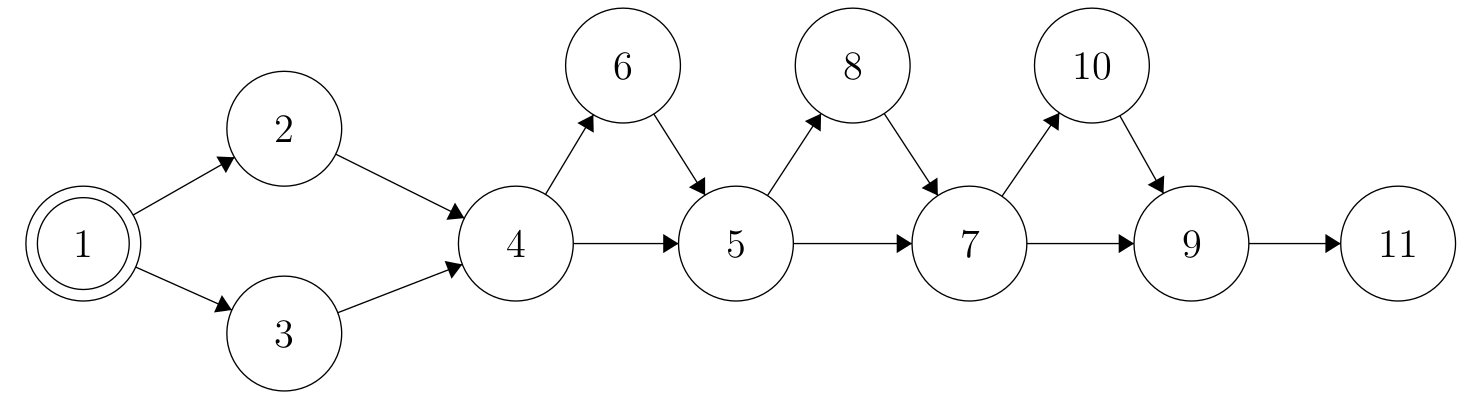
\includegraphics[width=\figwidth\columnwidth]{images/fabrikant/graph.jpg}
	\caption{Fabrikant graph representation}
	\label{fig:fabr_graph}
	\vspace{\figvspace}
\end{figure}

Node 1 represent the only source of traffic, node 4 will prefer to reach the 
destination through node 2, but the link is slower, triggering changes in the
network as required by \cite{fabrikant}.

Taking this base frabrikant graph other 4 graphs has been deveolped, one for each
\ac{MRAI} strategy applyed.

\subsection{Clique Graph}
\label{subsec:clique_graph}

The clique graph used for the clique experiemnts is composed of \num{15} nodes
plus one external node that is the source of a destination.
Each node is connected to every other node in a mesh network. The only node that
does not respect this rule is the destination source. it has only one link 
that is connected to the node of the mesh network number \num{0}.

Relationships between nodes are of the servicer type, so each node has \num{14}
clients to updated when it receives an update.
This ensures that the information is shared in the entire network.

For this network has been generated one graph for each fixed \ac{MRAI} used, so
that at the end we had \num{60} different clique graphs with the correct timer value
equal on each link.

\subsection{Internet Like Graph}
\label{subsec:internet_graph}

This network is composed of \num{100} nodes, it is not enough to emulate the Internet
but, with enough computation time, the results should be comparable with bigger graphs.
The graph has been produced following \cite{elmokashfi}.

In the graph has been chosen only one node that shares a destination.
The node has been chosen randomly in the set of clients nodes.

For each experiment, depending on the type of \ac{MRAI}, a new graph file has
been generated with different MRAIs values on the edges.

In total has been generated \num{6000} internet like graphs.

\section{Input arguments}
\label{sec:envDesc}

In this section are described the inputs arguments used for the different environments.

\subsection{Fabrikant arguments}
\label{sec:fabrikant_arguments}

\begin{itemize}
	\item seeds: \num{20} different seeds;
	\item Signaling: "AWA", The input signal determines the messages that 
		the source should send
	\item Implicit withdraw: active
	\item Withdraw distributions: \num{3} different withdraw uniform distributions
		$[5, 10]$, $[10, 15]$ and $[30, 45]$
	\item Reannouncement distributions: \num{3} different announcement uniform distributions
		$[5, 10]$, $[10, 15]$ and $[30, 45]$
	\item Processing time: constant with value \num{0.00001}
	\item Network delay: \num{3} uniform distributions in $[0.001, 1]$, $[0.5, 3]$ and $[2, 6]$
\end{itemize} 

The number of possible different combinations of these values is \num{540}, so 
for each different \ac{MRAI} type has been done \num{540} experiments and
in total \num{2160} expieriments in the fabrikant environment.

\subsection{Clique arguments}
\label{subsec:clique_arguments}

\begin{itemize}
	\item seeds: \num{10} different seeds;
	\item Signaling: "AW" 
	\item Implicit withdraw: active
	\item Withdraw distributions: uniform distribution $[5, 10]$
	\item Reannouncement distributions: Ininfluent 
	\item Processing time:i uniform distribution $[0.01, 1]$ 
	\item Network delay: uniform distribution in $[0.012, 0.1]$
\end{itemize} 

This environment attempt to replicate what has been presented in \cite{griffin2001experimental}

In total this environment would run 10 different permutations because the only
element that can differ is the input seed.
But has been done in a total of \num{61} experiments changing the \ac{MRAI} value between
$0$ and $60$, so in total, we had \num{610} runs, \num{10} for each \ac{MRAI} value.
It wouldn't have much sense, in my opinion, to run more than one simulation batch per
\ac{MRAI} value, because the repetition of the seed with no difference in any
other parameter would have produced the same result.

\subsection{Internet like arguments}
\label{subsec:internet_like_arguments}

\begin{itemize}
	\item seeds: \num{10} different seeds;
	\item Signaling: "A" 
	\item Implicit withdraw: active
	\item Withdraw distributions: Ininfluent
	\item Reannouncement distributions: Ininfluent 
	\item Processing time: constant with value \num{0.00001}
	\item Network delay: uniform distribution in $[0.012, 3]$
\end{itemize} 

The environment has been used for random experiments and fixed mrai experiments.

Like in the clique experiments, in the case of the fixed \ac{MRAI}, every link
had the same timer value.
But this time has been used also fractions of seconds to highlight the trend.
There have been \num{121} experiments with \ac{MRAI} in the ensemble $[0.0, 60]$.
In the first fraction $[0.0, 5.0]$ has been used a step of \num{0.1} doing \num{51}
experiments.
The second fraction was $[5.5, 20]$ with a step of \num{0.5}, doing in total \num{30}
experiemnts.
The last subset was $[21, 60]$ with a step of \num{1}, doing in total \num{40}
experiments.
The final total is \num{121} experiments and for each of them has been done
\num{10} runs, one for each possible seed of the environment.

The second type of experiments with the internet like environment were run 
with random graphs.
Before running a random experiment the $MRAI_{mean}$ were chosen randomly before
the generation of the random graph.
In total has been chosen \num{60} random $MRAI_{mean}$ uniformly distributed
in the set $[0, 60]$ the limit \num{60} has been chosen arbitrarily being the
double of the actual standard.
\num{100} random graphs were generated for each $MRAI_{mean}$.
Each link would obtain a random value in the set $[0, 240]$ and then all the
values would be re-proportioned to respect the $MRAI_{mean}$
At the end for each random graph would be done \num{10} runs thanks to the 10 
different seeds.
The total number of this particular configuration is $60*100*10$ equal to 
\num{60000} single runs 

\section{Experiments Results}
\label{sec:results}

The first results that I would like to examine is the single node
results from the fabrikant experiment.
In \Cref{fig:fabr_30sec_9_signaling,fig:fabr_descendent_9_signaling} are represented
two signalling outputs of the node number \num{9}.

The $x$ axis represents the number of messages in the output signal.
The first $y$ axis, the one on the left, represents the probability to have a certain
number of messages in the output sequence and should be used with "withdraw
messages", "Advertisement messages" and "Total messages" lines.
For example in \Cref{fig:fabr_30sec_9_signaling} we can see that there is a really
high probability to have \num{0} withdraws in the output sequence, and we would never
see more than 1 withdraw by the fact that the "withdraw line" doesn't go over that
value of the $x$ axis.
In the same way, we can read the other lines, for example in the same figure is
possible to see that the more probable output signal is composed by \num{3} messages,
because is the highest point of the blue line.
The second $y$ axis, the one on the right, represents the number of \textbf{unique}
states.
This axis should be used with the line that represents the "possible outputs".
Looking the \Cref{fig:fabr_30sec_9_signaling} is possible to see that for
output signals with \num{6} messages we have more than \num{40} uniques output
states.

Knowing that the output signalling is strictly dependent by the input that a 
node receives and the evaluation time of those messages we can already see the
effects of an inconvenient \ac{MRAI} setting.
In \Cref{fig:fabr_descendent_9_signaling} there are a lot more output states.
In those experiments we reach event output states of length \num{16} and the 
probability to have at least one withdraw is higher to the probability to 
don't have one.
Knowing that the implicit withdraw system is active having one withdraw means
that the node has no other possibilities to withdraw the network not knowing any
other path.

\begin{figure}[tb]
	\centering
	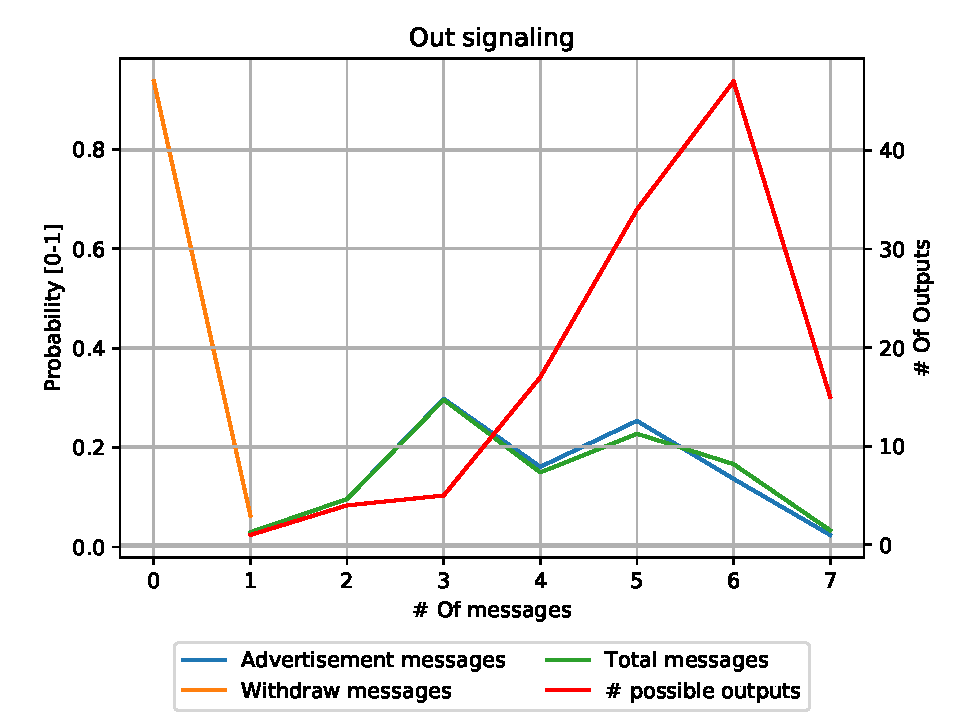
\includegraphics[width=\figwidth\columnwidth]{images/fabrikant/fabrikant-30fixed/results_9_signaling_nmessage_prob}
	\caption{Fabrikant MRAI fixed 30 seconds, node 9 signalling output}
	\label{fig:fabr_30sec_9_signaling}
	\vspace{\figvspace}
\end{figure}

\begin{figure}[tb]
	\centering
	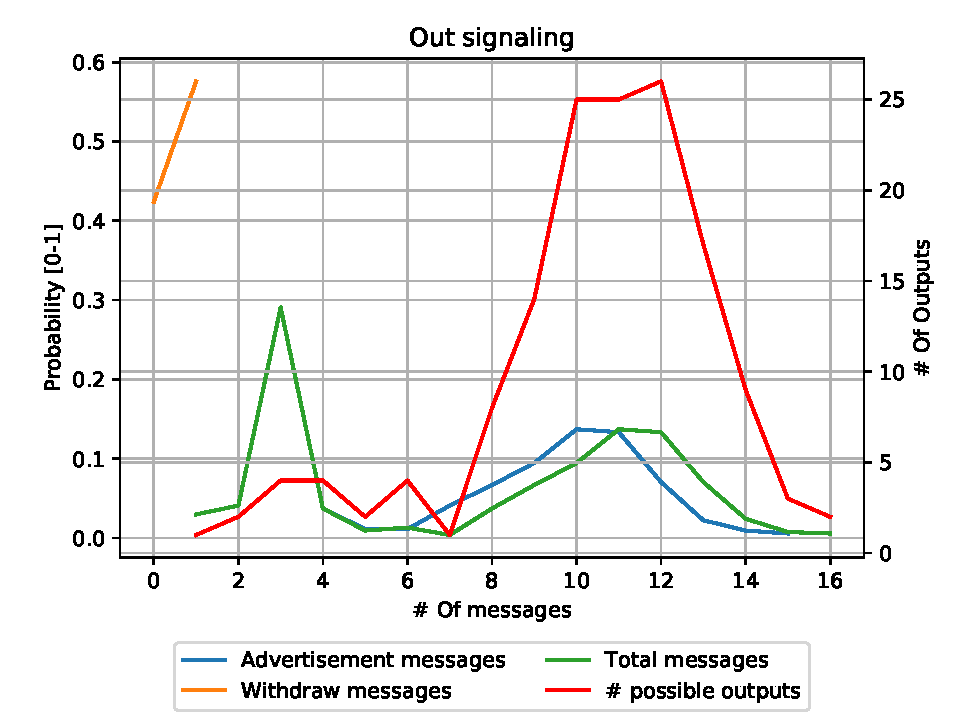
\includegraphics[width=\figwidth\columnwidth]{images/fabrikant/fabrikant-descendent/results_9_signaling_nmessage_prob}
	\caption{Fabrikant MRAI descendent, node 9 signalling output}
	\label{fig:fabr_descendent_9_signaling}
	\vspace{\figvspace}
\end{figure}

Like we said before we used 4 different \ac{MRAI}s strategies in the fabrikant
environment, and them are compared in the \Cref{fig:fabr_conv_time_comp,fig:fabr_msg_comp}.
The no mrai method is strictly dependent on delays and other events of the network
and is possible to see that it has the smallest convergence time but with the higher
number of messages necessary to reach the convergence.
The \num{30} seconds strategy could be the slowest one because if something goes
wrong is necessary to wait a long time to repair the damage, but it wouldn't
require too many messages on the other side.
The descendant method seems a good solution on the convergence time side, but
on the other side, like is described in \cite{fabrikant} it could easily lead
to a lot of messages.

\begin{figure}[tb]
	\centering
	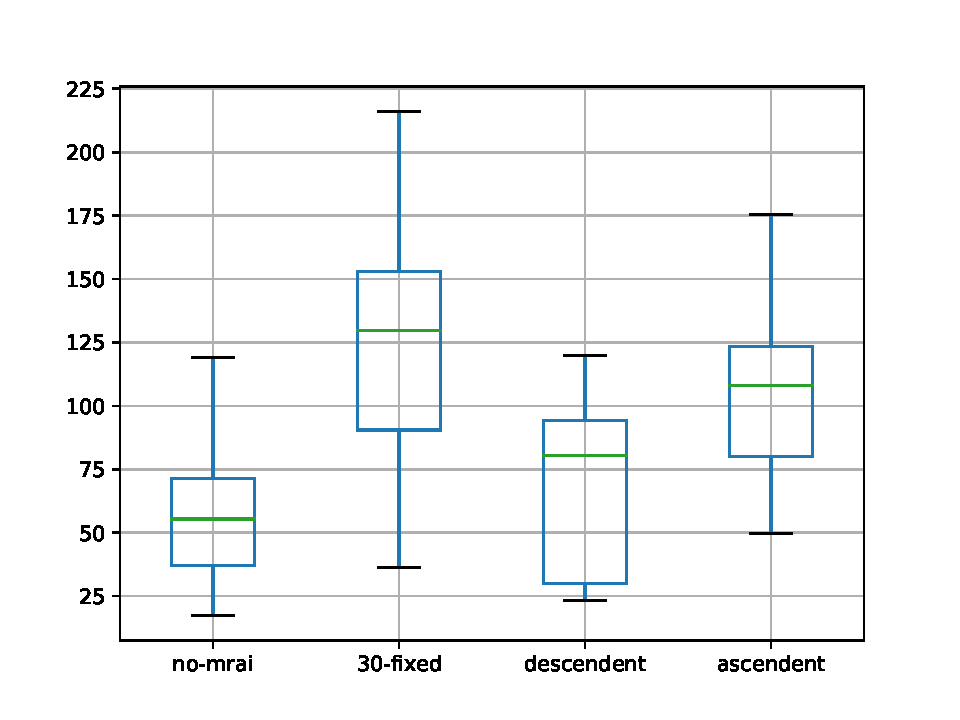
\includegraphics[width=\figwidth\columnwidth]{images/fabrikant/convergence_time}
	\caption{Fabrikant experiments convergence time comparison}
	\label{fig:fabr_conv_time_comp}
	\vspace{\figvspace}
\end{figure}

\begin{figure}[tb]
	\centering
	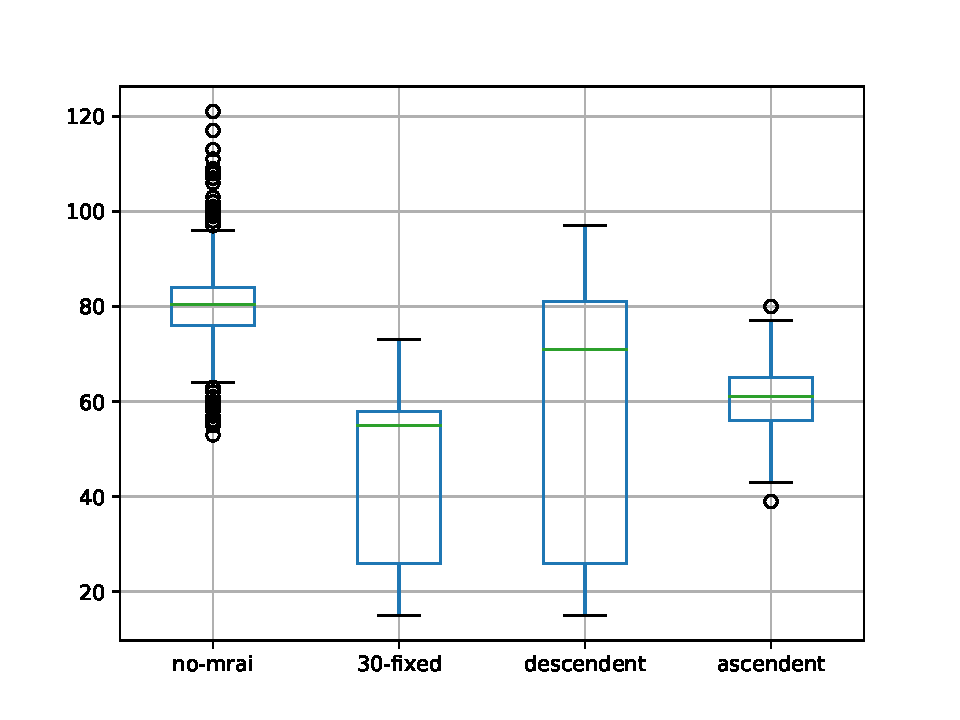
\includegraphics[width=\figwidth\columnwidth]{images/fabrikant/messages_comparison}
	\caption{Fabrikant experiments number of messages comparison}
	\label{fig:fabr_msg_comp}
	\vspace{\figvspace}
\end{figure}

In \Cref{fig:clique_pareto_freq,fig:clique_mrai_evolution} are reported the general
network results obtained in the clique environment.
The goal of this study is to see in a general way how \ac{MRAI} could influence
even a small network as this clique of \num{15} nodes.

In \Cref{fig:clique_pareto_freq} every point of the plot is the mean of the \num{10}
runs executed with a fixed \ac{MRAI}.
On the $x$ axis is represented the number of messages correlated with the convergence
time on the $y$ axis.
The red points are the Pareto front of the set of all points.
We can see from the plot that a lot of experiments has a mean of messages sent 
around \num{2000} independently from the \ac{MRAI} so we can guess that after
a threshold of \ac{MRAI} the number of messages stabilizes around that value.
On the other side, before this threshold we can guess there is a lot of variance
in the number of messages but the mean convergence time is similar.
These guesses are confirmed by the \Cref{fig:clique_mrai_evolution} where we can clearly
see those trends.
The two $y$ axis are used to represent the trend of the convergence time and
the number of messages transmitted in relation of the \ac{MRAI} value.

\begin{figure}[tb]
	\centering
	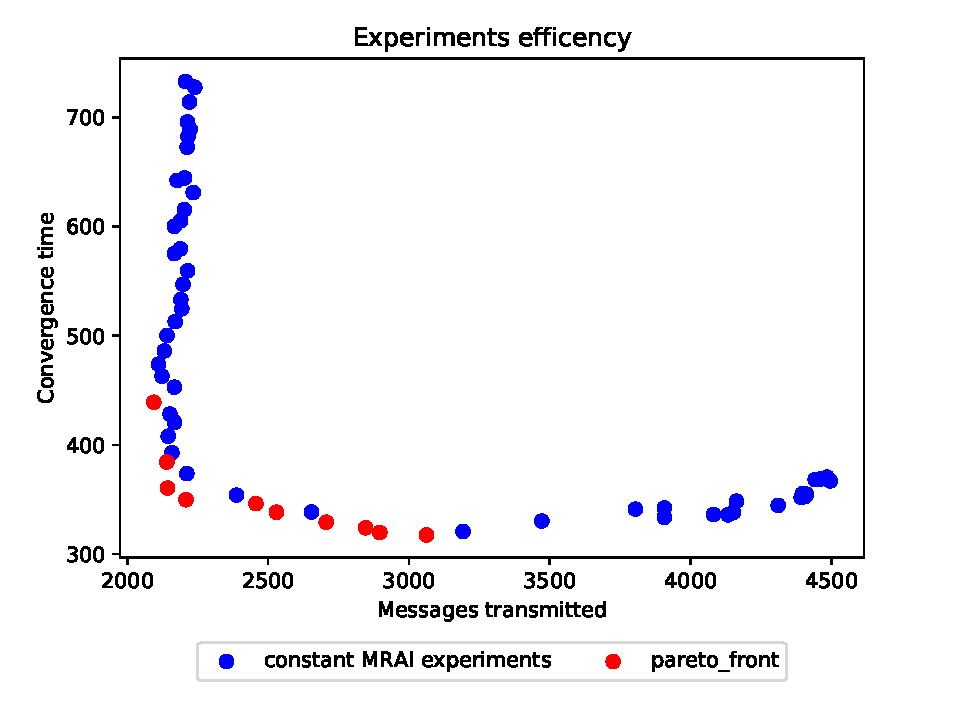
\includegraphics[width=\figwidth\columnwidth]{images/clique/pareto-clique-constant}
	\caption{Pareto front in the clique environments}
	\label{fig:clique_pareto_freq}
	\vspace{\figvspace}
\end{figure}

\begin{figure}[tb]
	\centering
	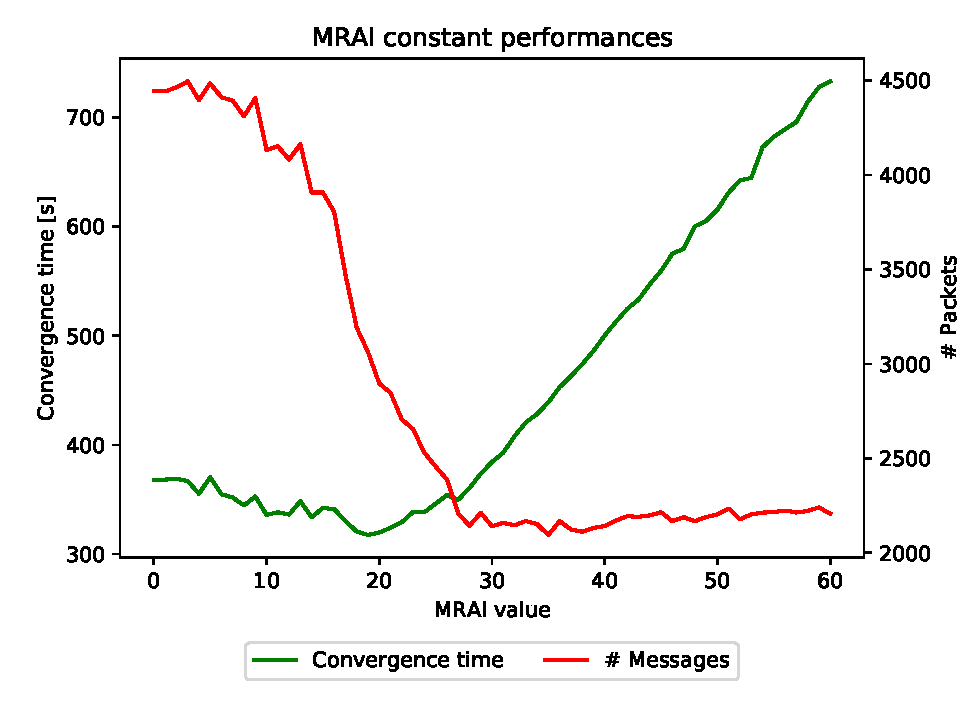
\includegraphics[width=\figwidth\columnwidth]{images/clique/mrai_evolution}
	\caption{Evolution of the number of messages sent and the convergence time as \ac{MRAI} grows
		in the clique environment}
	\label{fig:clique_mrai_evolution}
	\vspace{\figvspace}
\end{figure}

The next experiment that I would like to study is the fixed \ac{MRAI} strategy
on the internet like environment.
The two \Cref{fig:constant_mrai_pareto_freq,fig:constant_mrai_evolution} have the
same structure of the clique results but this time we can see a lot fewer messages
transmitted to reach the convergence.
Also this time we can see in \Cref{fig:constant_mrai_pareto_freq} that a lot of
experiments are concentrated in the range between \num{320} and \num{340} messages
with a high variance on the convergence time.
In fact, we can see from \Cref{fig:constant_mrai_evolution} that the trend is similar
to the one that we saw in the clique graph, but this time the "transmitted messages" line
has a steep fall, it reaches the constant state in few seconds (the clique experiment
in \Cref{fig:clique_mrai_evolution} took more than \num{20} seconds).
But we can say the same thing for the convergence time too.
Tose results are similar to the one available in \cite{griffin2001experimental}.

\begin{figure}[tb]
	\centering
	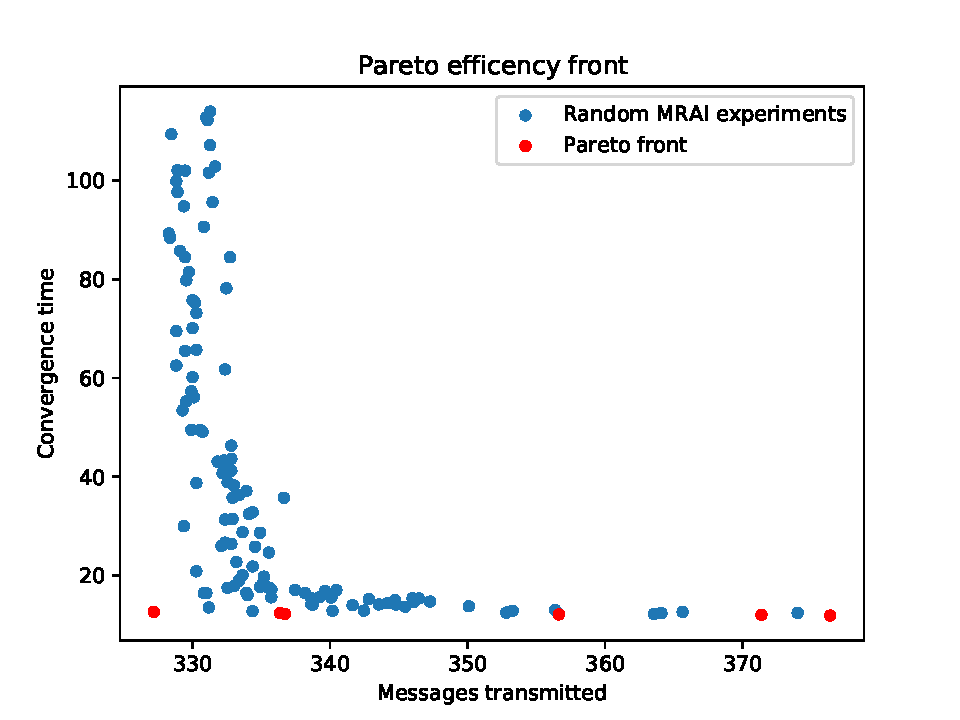
\includegraphics[width=\figwidth\columnwidth]{images/internet_like/graph-100-constant/pareto-constant}
	\caption{Pareto front in the Internet like constant \ac{MRAI} environment}
	\label{fig:constant_mrai_pareto_freq}
	\vspace{\figvspace}
\end{figure}

\begin{figure}[tb]
	\centering
	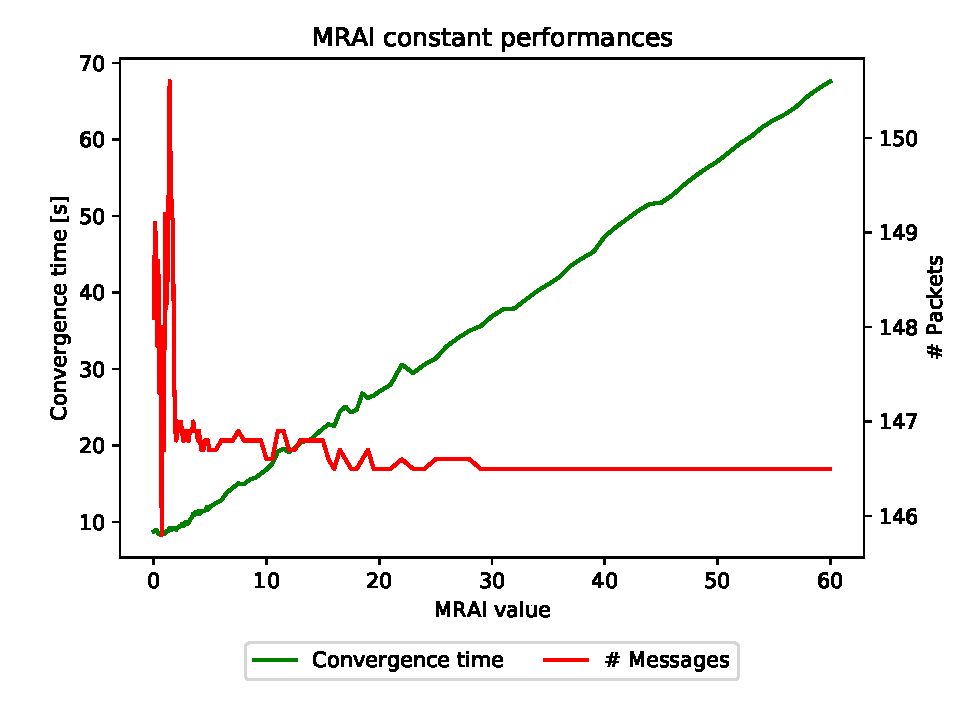
\includegraphics[width=\figwidth\columnwidth]{images/internet_like/graph-100-constant/mrai_evolution}
	\caption{Evolution of the number of messages sent and the convergence time as \ac{MRAI} grows
		in the internet like constant \ac{MRAI} environment}
	\label{fig:constant_mrai_evolution}
	\vspace{\figvspace}
\end{figure}

Some more general results could be saw taking into consideration the random \ac{MRAI}
strategy on the internet like graph.
The results are visible in \Cref{fig:random_mrai_pareto_freq}.
The first thing that we can see is that this time there are not huge spikes 
for certain messages amount.
The number of messages sent is more distributed between \num{300} and \num{360}.
Also, the convergence time is more distributed, thanks to the random \ac{MRAI} distribution.
We can guess that if a central node has a huge \ac{MRAI} timer and it transmits
incorrect information it would act as a bottleneck for the update with the 
correct information.

\begin{figure}[tb]
	\centering
	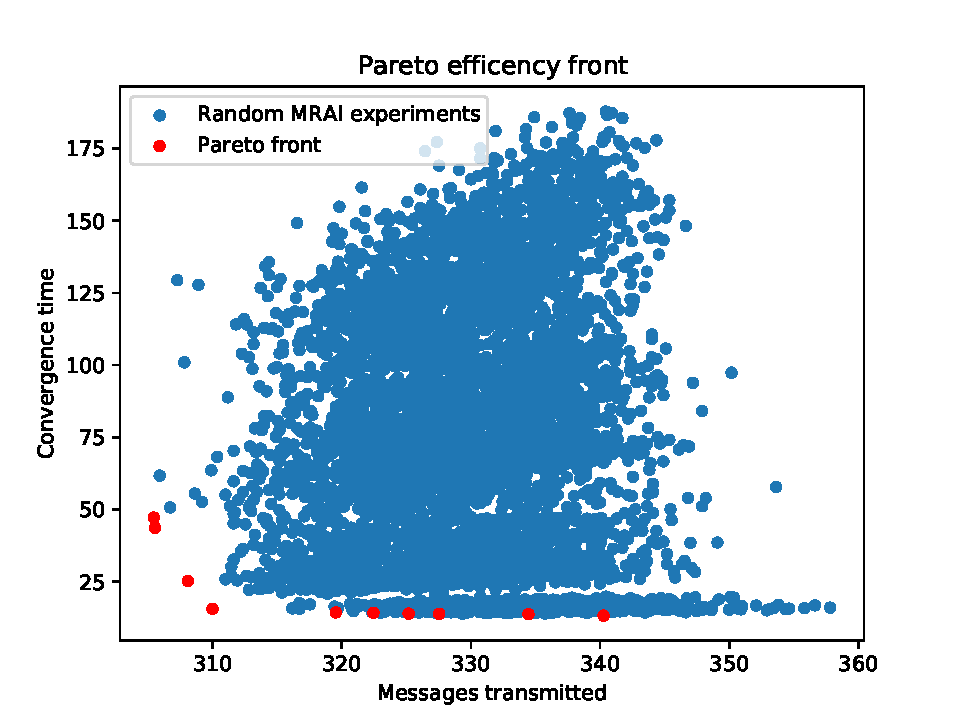
\includegraphics[width=\figwidth\columnwidth]{images/internet_like/graph-100-random/random-multiple_mrais}
	\caption{Pareto front in the Internet like random environment}
	\label{fig:random_mrai_pareto_freq}
	\vspace{\figvspace}
\end{figure}

From the comparison of the two \ac{MRAI} strategies we can see in \Cref{fig:internet_pareto_comparison}
that the constant \ac{MRAI} cover a really small part of the random strategy.
And for small values of \ac{MRAI} is also possible for the constant strategy
to send more messages than the random one.

\begin{figure}[tb]
	\centering
	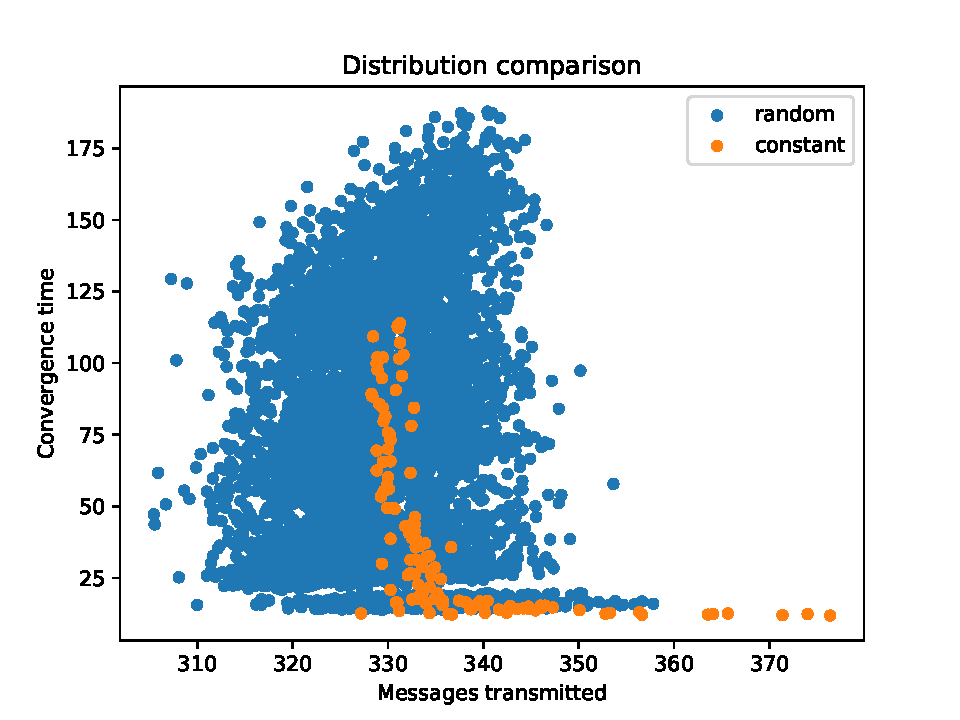
\includegraphics[width=\figwidth\columnwidth]{images/internet_like/combine_results_2}
	\caption{Comparison of the random strategy and the constant one in the internet like environment}
	\label{fig:internet_pareto_comparison}
	\vspace{\figvspace}
\end{figure}

\bibliographystyle{IEEEtran}
\bibliography{references}

\end{document}
